\chapter{Grundlagen der angewandten Ethik und Moral}\label{chap:grundlagen_ethik}
Im Folgenden erfolgt eine Begriffsdefinition und Abgrenzung der Begriffe Ethik und Moral, welche als Grundlage für die in \autoref{sec:def_ethischer_werte} definierten Werte dient.
Im Rahmen dieser Arbeit wird insbesondere die angewandte Ethik betrachtet, da die spätere Konzeption des Vorgehens der Entwicklung einer Reinforcement-Learning-Anwendung stark praxisorientiert erfolgt.

\begin{figure}[h]
    \centering
    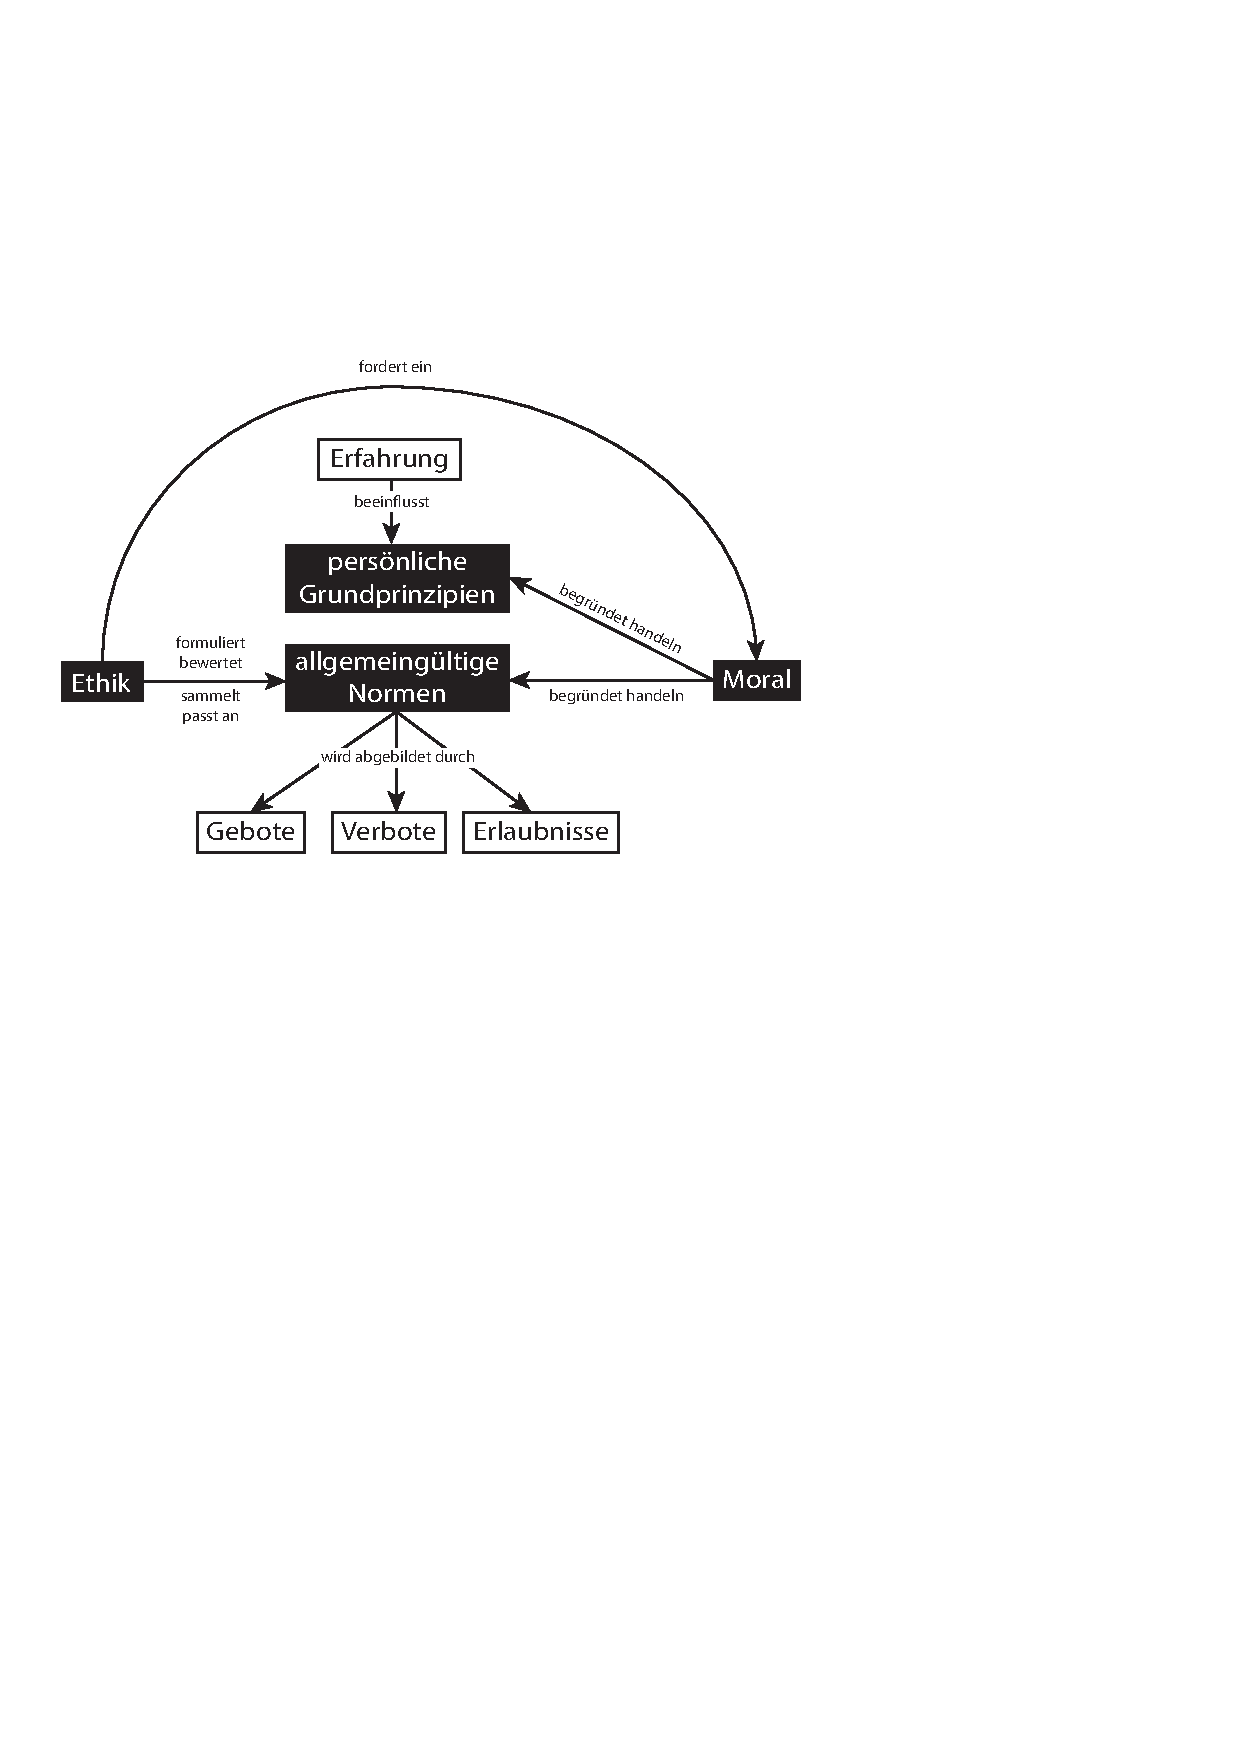
\includegraphics{graphics/ethik_overview.png}
    \caption{Überblick über die Beteiligten Komponenten des moralischen Handelns und dessen Zusammenhang.}
    \label{fig:ethik}
\end{figure}

Sowohl Ethik als auch Moral befassen sich mit Normen, welche in diesem Kontext als \enquote{[...] allgemeingültige Regeln [...]} \cite[S. 10 ff.]{schicha2010} beschrieben werden.
Die angewandte Ethik beschreibt dabei die Formulierung und Bewertung praxisbezogener Normen.
Im Gegensatz zu praxisbezogenen Normen stehen Idealnormen als wünschenswerte aber praktisch nicht umsetzbare Werte.
Als Disziplin der Philosophie fordert die Ethik, wie in \autoref{fig:ethik} abgebildet, nicht nur das Handeln gemäß der Normen ein, sie dient ebenfalls als Sammlung der Gesamtheit aller Normen.
Nicht zuletzt stellt die Ethik auch die Grundlage für die Findung und Anpassung der Normen durch zwischenmenschlichen Diskurs in den Vordergrund.
Auch wenn versucht wird, diesen Prozess rational zu begründen, kann eine Korrektheit nicht, wie etwa in naturwissenschaftlichen Disziplinen, nachgewiesen werden.
Als Wissenschaft ist die Ethik unabhängig von Autoritäten, sondern basiert auf \enquote{[...] Kriterien der Rationalität, der Begründung und der Verallgemeinerungsfähigkeit [...]} \cite[S. 22]{schicha2010}.
Anders verhält sich die Gültigkeit von Normen im Bezug auf den aktuellen Zeitgeist \cite[S. 10]{tannsjo2008}.
Normen können zu jedem Zeitpunkt ihre Gültigkeit verlieren, was jedoch ihre gegenwärtige Gültigkeit und Relevanz nicht einschränkt.
Auf persönlicher Ebene ergeben sich Werte und Normen aus persönlichen Erfahrungen und Interessen \cite[S. 3f]{mcnaughton1988}, was jedoch im Laufe des Lebens von äußeren Einflüssen, wie Religionen und unserer direkten Umwelt beeinflusst wird.
\ab 
Moral bzw. moralisches Handeln ist als praktische Anwendung der, durch die Ethik diskutierten Normen \cite[S. 80]{werkener2017} anzusehen.
Die allgemeingültige Anwendung und Zusicherung von Normen zum Zwecke des moralischen Handelns erfolgt durch Grundprinzipien \cite[S. 11]{schicha2010}, die es ermöglichen auch in vorher unbekannten Situationen gemäß der Normen moralisch zu handeln.
Normen können durch \enquote{[...] Gebote, Verbote und Erlaubnisse [...]} \cite[S. 80]{werkner2017} abgebildet und über die persönliche Moral hinaus formuliert und eingefordert werden.
Sie finden speziell dann Anwendung, wenn das Handeln nicht allein durch die Intuition entschieden werden kann.

\section{Maschinenethik und Einordnung von Reinforcement-Learning-Agenten}
Durch die Komplexität des menschlichen Lebens und Handelns ist es in der angewandten Ethik nur schwer möglich, Normen für jede Situation zu definieren, die allgemeingültig anwendbar sind und dennoch möglichst viele Fälle abbilden.
Deshalb haben sich Bereitsethiken entwickelt, die explizit ein Teilgebiet des menschlichen Lebens abbilden.
Bereichsethiken sind nicht unbedingt auf spezielle Verfahren oder Technologien, sondern viel mehr auf übergeordnete Anwendungen und ethische Fragen eines Systems bezogen.
Ethik ist jedoch kein festgeschriebenes Regelwerk, weswegen im Rahmen dieser Arbeit für die Definition ethischer Werte eine Abstraktion und Generalisierung der verwandten Bereichsethiken und allgemeingültiger Normen erfolgt.
\ab 
Inhaltlich besitzt die Maschinenethik \cite[S. 6]{rath2019} eine größe inhaltliche Nähe zur Thematik des Reinforcement Learning, indem die Anwendungen und ethischen Fragestellungen Überschneidungen aufweisen.
Die Maschinenethik als solche beschreibt zum einen das Verhalten der Menschen im Bezug auf Maschinen und zum anderen, insbesondere im Kontext der lernenden Systeme, das moralische Handeln von Maschinen.
Handeln Agenten z.B. durch die Begrenzung der Fähigkeiten und des Kontextes nicht implizit moralisch, so müssen Normen explizit für die Berücksichtigung in Maschinen  technisch abgebildet werden \cite[S. 34]{bendel2019}.
Dem Agenten soll es dann möglich sein eigenständig in unbekannten Situationen moralisch zu Handeln.
Als Teilgebiet der Ethik ist neben der Umsetzung und Konzeption der Normen auch die Bewertung des Handelns zu betrachten, insbesondere mit dem Ziel das Handeln des Agenten unseren Erwartungen menschlicher Moral zu entsprechen.
Grundlage der Betrachtung explizit ethischer Agenten ist die Frage, ob Maschinen überhaupt moralisch Handeln können.
Laut \cite[S. 41 ff.]{bendel2019} ist die Handlungsfähigkeit als Grundlage des moralischen Handelns an die Fähigkeit zur \enquote{[...] Orientierung an Gründen [...]} \cite[S. 41]{bendel2019} und an die \enquote{[...] Selbstursprünglichkeit [...]}\cite[S. 42]{bendel2019} gekoppelt.
Die Erfüllung dieser Bedingungen ist dabei abhängig von Art und Implementierung eines Systems.
Damit eine Maschine also explizit moralisch handeln kann, muss sie zumindest grundlegend wie ein Mensch handeln.
Die Fähigkeit zur Orientierung an Gründen erfüllen Maschinen, sobald ihr Verhalten an die Erfüllung eines Zieles gebunden oder zumindest dadurch motiviert ist.
Zur Erfüllung der Selbstursprünglichkeit fordert \cite{bendel2019} die Eigenschaften Interaktivität, basale Autonomie und Adaptivität.
Interaktivität und Adaptivität beschreiben dabei die Fähigkeit der Reaktion bzw. der Anpassung des Verhaltens auf äußere Einflüsse und basale Autonomie die Änderung des Zustands ohne äußere Einwirkung.
Erfüllt ein System diese Eigenschaften, so besitzt es zumindest Handlungsfähigkeit und kann, wenn die Gründe für das Handeln einer Moral entsprechen auch moralisch handeln.
\ab 
Im Bezug auf die Thematik des Reinforcement Learning besitzen die daraus entstehenden Agenten eine Orientierung an Gründen, indem die Belohnungsfunktion und das daraus resultierende Ziel die Belohnung zu maximieren das Verhalten beeinflussen.
Zur Erfüllung der Selbstursprünglichkeit müssen zudem Interaktivität, basale Autonomie und Adaptivität betrachtet werden.
Reinforcement-Learning-Agenten können im Sinne der Interaktivität auf äußere Einflüsse reagieren und das eigene Verhalten gemäß der Adaptivität ebenfalls anpassen.
Indem die Agenten einen eigenen Antrieb haben, auch ohne äußere Einflüsse Zustände zu verändern ist auch die basale Autonomie vorhanden.
Dadurch lässt sich darauf schließen, dass Reinforcement-Learning-Agenten zumindest ein gewisses Maß an Handlungsfähigkeit besitzen.
Damit die Agenten nun auch explizit moralisch handeln können, muss die Grundlage des Handelns auf Normen basieren.
Insbesondere in der in \autoref{sec:massnahmen} vorgestellten Maßnahmen zur Entwicklung von ethischen Reinforcement-Learning-Agenten wird die Umsetzung des moralischen Handelns der Agenten auf die in \autoref{sec:def_ethischer_werte} definierten Normen bzw. Werten bezogen.
